\documentclass[10pt,twocolumn,letterpaper]{article}
\usepackage[margin=0.75in,columnsep=0.25in]{geometry}
\usepackage{mathptmx}
\renewcommand{\ttdefault}{pcr}
\usepackage[T1]{fontenc}
\usepackage{microtype}
\usepackage{booktabs}
\usepackage{url}
\usepackage[hidelinks]{hyperref}
\usepackage{listings}
\usepackage{xcolor}
\usepackage{cite}
\usepackage{balance}
\usepackage{graphicx}
\lstset{basicstyle=\ttfamily\footnotesize,breaklines=true,columns=fullflexible,frame=single,framerule=0.3pt}
\setlength{\parskip}{0pt}
\raggedbottom
\title{\Large\bfseries PyPI API Drift: A Release-Level Record of Public API Changes\\in 1,872 Popular Python Libraries, with a Checker and a Benchmark\\for Version-Aware Code Generation}
\author{Pushkar Devanahalli Gopalakrishna\\Independent Researcher, USA}
\date{}
\begin{document}
\maketitle

\begin{abstract}
Ask a code assistant to append a row to a pandas DataFrame and it may write \texttt{df.append(row)}, a method removed
in pandas 2.0. Models trained on code from many releases cannot tell which API exists in the version a user has
installed, and benchmarks of this problem are small and frozen. We present \emph{PyPI API Drift}, a release-level
record of the public APIs of the 1,872 most-downloaded Python libraries: up to 80 recent final releases each
(55,565 releases, 2021--October 2026), with signatures, 15,258,652 release-to-release changes and
210,535 deduplicated breaking changes. Extraction is static and import-free, reads only the
needed bytes of each wheel, separates names that were truly removed from names that merely left the documented API,
and marks with confidence labels and a coverage layer where static analysis cannot see. It is a high-precision,
low-recall record: in two held-out runtime audits by AI agents isolated from the pipeline (on earlier data versions),
88.8\% and 91.9\% of high-confidence breaking changes were confirmed, while recall over all runtime-visible changes is limited (16 of
99). On top of it we release an offline checker, lookup tools with a Model Context Protocol (MCP) server for coding agents, and
VersionProbe, a benchmark of 10,958 valid/invalid snippet pairs. In a preregistered code-repair experiment,
repeated across 4 models from one model family, API history from the dataset raised the share of API-compatible,
intent-preserving migrations (under our evaluation protocol) to 68.5\%--69.9\% for every model, from
7.0\%--56.6\% unaided and 46.2\%--62.2\% with the new release's documentation.
13.4\% of patch releases contain at least one breaking change.
\end{abstract}

\section{Introduction}
Python libraries evolve quickly. Functions are deprecated and removed, parameters are renamed or made
keyword-only, and modules are reorganized. For developers this causes upgrade failures; for LLM-based code
assistants it causes a subtler failure: models trained on a mix of old and new code confidently produce calls that
are valid for some version of a library but not the one installed. Typical examples include
\texttt{DataFrame.append} (removed in pandas 2.0), \texttt{read\_csv(error\_bad\_lines=...)},
\texttt{Retry(method\_whitelist=...)} (removed in urllib3 2.0) and \texttt{from flask import escape} (removed in
Flask 3.0).

Recent benchmarks measure this weakness \cite{versicode,gitchameleon,gitchameleon2,wang2024deprecated}, but they
are small, hand-curated or frozen at a point in time. What is missing is \emph{infrastructure}: a large, accurate,
continuously refreshable record of which public API existed in which release of which library. This paper
contributes:
\begin{itemize}\setlength\itemsep{0pt}
\item \textbf{A dataset} of public-API snapshots and changes for 1,872 libraries and 55,565 releases,
with signature-level detail, deduplication across inheritance and re-exports, confidence labels and a coverage layer
that marks where static analysis cannot see (Sections~\ref{sec:method}--\ref{sec:dataset});
\item \textbf{An extraction method} that is cheap (range reads of only the Python members of wheels), import-free,
and conservative about what counts as a removal (Section~\ref{sec:method});
\item \textbf{Tools}: \texttt{apidrift-check}, a version-aware checker for Python code; \texttt{apidrift-lookup} and an
MCP (Model Context Protocol) server that give coding agents the same record; and \textbf{VersionProbe}, a paired benchmark of 10,958
valid/invalid snippet pairs (Section~\ref{sec:tools});
\item \textbf{A validation} by runtime audits that AI agents isolated from the pipeline carried out of precision, benchmark labels and recall, a comparison
with two existing tools, and real upgrade failures (Section~\ref{sec:validation});
\item \textbf{An evaluation of the record's effect on code models}: a preregistered code-repair experiment, repeated across
4 models from one family (Section~\ref{sec:models});
\item \textbf{Findings} on breaking changes and semantic versioning in the Python ecosystem (Section~\ref{sec:findings}).
\end{itemize}
The dataset was built in successive versions (v1.0 to v1.3), each fully re-extracted after audits exposed
systematic errors; Appendix~\ref{sec:history} lists the changes. Figures describe the released version
(2026.10-v1.3); Appendix~\ref{sec:history} also lists the version each validation study and experiment
used.

\section{Related Work}
\textbf{Version-aware code generation.} VersiCode~\cite{versicode} covers over 300 libraries and 2,000 versions
up to 2023, labelling API changes at the name level. GitChameleon~\cite{gitchameleon} and GitChameleon~2.0
\cite{gitchameleon2} provide 116 and 328 executable, version-conditioned problems. Wang et
al.~\cite{wang2024deprecated} study deprecated API usage by LLMs over 145 API mappings in eight libraries. Our work
is complementary: it supplies signature-level API records across far more libraries and recent releases, from
which such benchmarks can be generated and refreshed.

\textbf{API evolution and breaking changes.} AexPy~\cite{aexpy} detects breaking changes in Python packages by
combining static and dynamic analysis; it imports each release. griffe~\cite{griffe} loads Python APIs statically
and reports breaking changes between two versions, for documentation and release checks. Section~\ref{sec:recall}
compares both with this dataset on the same release pairs. In the Java ecosystem, Raemaekers et al.~\cite{raemaekers2014}
reported that about one third of Maven releases introduce a breaking change, regardless of version increment, while
Ochoa et al.~\cite{ochoa2022} found higher semantic-versioning compliance in a later replication. We provide a large,
open, release-level dataset for Python, together with measured precision.

\section{Method}\label{sec:method}
\subsection{Release selection}
We take the top 2,000 projects by recent downloads from the public top-PyPI-packages list (October 2026),
and for each the final (non-pre-release, non-yanked) releases uploaded since 2021-01-01 that ship a wheel,
capped at the 80 most recent releases per project. For every release we pick one wheel, preferring a pure-Python
wheel, then a CPython \texttt{manylinux} x86\_64 wheel for the newest interpreter. Releases are ordered by version
number; placeholder versions (\texttt{0.0.0}, \texttt{0}, \texttt{0.0}) uploaded after a project's real releases are
excluded, because version order would place them first and diff them against unrelated builds. This yields
55,839 releases of 1,872 projects (83.5\% pure-Python wheels), of which 55,565 were analysed
(274 releases of packages with more than 8,000 modules were skipped); 1,869 projects have
at least one analysed release.

\subsection{Range reads}
Wheels are ZIP files. We read the end-of-central-directory record and the central directory with HTTP range
requests, select \texttt{.py} and \texttt{.pyi} members (excluding \texttt{tests}, \texttt{test},
\texttt{conftest} and metadata), and fetch only members whose CRC changed since the previous release of the same
project. Replaying this fetch logic over the full histories of 300 randomly chosen projects
(8,149 releases) downloads 8.5\% of the wheels' bytes (95\% bootstrap CI 5.7--14.7\% over
projects), about 26\,GB (17--44\,GB) for the whole dataset instead of the 300\,GB needed to
download every wheel. The saving comes from wheels of 1\,MB or more (95.3\% of the bytes, of which
5.3\% is fetched); small pure-Python wheels consist mostly of the files we need anyway (74.1\%
fetched). The median release costs 81\,KB and two requests, and only 15.2\% of
\texttt{.py}/\texttt{.pyi} members have to be fetched at all.

\subsection{Static extraction}
Each module is parsed with Python's \texttt{ast}; nothing is imported or executed, so untrusted package code never
runs. Per module we record definitions (functions with full signatures, classes with members, including instance
attributes set through \texttt{self}), imports, star imports, a statically evaluable \texttt{\_\_all\_\_}, and the
behaviour of a module-level \texttt{\_\_getattr\_\_}. The extractor handles the Python idioms that most often mislead static analysis: conditional and \texttt{try/except} imports (fallback branches never
override the primary binding); PEP~484 positional-only parameters written as \texttt{\_\_x} (normalized to PEP~570
form); \texttt{@overload} declarations; runtime source taking precedence over \texttt{.pyi} stubs; names deleted with
\texttt{del}; classes created by calls (\texttt{TypedDict(...)}, \texttt{namedtuple(...)}); typing Protocols (members
excluded); namespaces populated dynamically (\texttt{globals()} writes, \texttt{exec}, protobuf builders), which are
treated as unknown; and classes whose constructor a decorator generates (\texttt{@dataclass}, attrs, factories), whose
inherited constructor signature is discarded.

\textbf{Module \texttt{\_\_getattr\_\_}.} Many libraries serve names lazily or through deprecation shims. A name counts
as served when \texttt{\_\_getattr\_\_} compares the requested name against a literal, or looks it up in a module-level
container whose contents can be followed statically (literals, \texttt{X["k"] = ...}, \texttt{X.update(...)} with a
literal or a comprehension over a literal list) \emph{and} the branch returns an object; it is marked deprecated when
that branch warns. A name the function explicitly rejects (e.g.\ NumPy's \texttt{\_\_former\_attrs\_\_}) is known to
be absent.

\textbf{Public API.} The public API of a release is the set of paths reachable from public modules (no
underscore-prefixed segment) through \texttt{\_\_all\_\_} or, when absent, public definitions and (in packages)
re-exports, resolved through relative imports, star imports and inheritance from classes defined in the same
distribution, plus names served by module \texttt{\_\_getattr\_\_}.

\subsection{Diffing, the accessibility test and confidence}
Consecutive releases are diffed per path. Signature changes are classified into \texttt{param\_removed},
\texttt{param\_renamed} (positional match), \texttt{required\_param\_added}, \texttt{became\_keyword\_only},
\texttt{became\_positional\_only}, \texttt{default\_removed}, \texttt{vararg\_removed}, \texttt{varkw\_removed} and
\texttt{positional\_reordered} (breaking), and several non-breaking types. The key design decision concerns removals:
a path that disappears from the public API is recorded as \texttt{removed} only if an \emph{accessibility test} on
the new release proves it unreachable by attribute access. If it is still reachable (e.g., dropped from
\texttt{\_\_all\_\_}, now an alias of an external object, served lazily) or reachability cannot be decided statically
(compiled modules, an open \texttt{\_\_getattr\_\_}), it is recorded once as non-breaking \texttt{left\_public\_api} and
carried forward. If it later becomes provably absent, the removal is recorded at that release; because the name may
already have been unavailable earlier, such removals are labelled medium confidence and their detail gives the earliest
possible release (NumPy dropped \texttt{float} in 1.24.0 but rejects it explicitly only from 1.24.2).

The same change often appears under every subclass and re-export path; one row per underlying change is flagged
\texttt{representative}, and counts in this paper use those rows. Changes are labelled \texttt{high} or
\texttt{medium} confidence; medium covers members missing from classes with bases in other packages, stub-derived
symbols, removed \texttt{**kwargs} or forwarded \texttt{*args}, classes rebound as aliases, constructor signatures of
decorator-built classes, and removals dated by provability as above.

\section{Dataset}\label{sec:dataset}
Table~\ref{tab:files} lists the released tables and Table~\ref{tab:types} the breaking changes by type. The data covers
55,565 analysed releases, 7,209,790 parsed modules (166 unparseable), 799,705
distinct signatures, 15,258,652 change events and 210,535 deduplicated breaking changes
(181,023 high-confidence; Fig.~\ref{fig:overview}). Each project's history covers at most its 80 most recent final
releases, so it is not a complete history of every release since 2021.

\begin{table}[t]\centering\small
\caption{Released tables (Parquet).}\label{tab:files}
\begin{tabular}{@{}lrl@{}}\toprule
File & Rows & Grain \\\midrule
releases & 55,839 & release \\
api\_history & 15,634,142 & path $\times$ state $\times$ release range \\
changes & 15,258,652 & change between releases \\
signatures & 799,705 & distinct signature \\
module\_coverage & 289,735 & module $\times$ coverage $\times$ range \\\bottomrule
\end{tabular}\end{table}

\begin{table}[t]\centering\small
\caption{Deduplicated breaking changes by type (high confidence). Kind changed: a symbol changed kind in a way that breaks callers, e.g.\ a method became a property.}\label{tab:types}
\begin{tabular}{@{}lr@{}}\toprule
Change type & Count \\\midrule
Symbol removed & 113,573 \\
Parameter removed & 21,068 \\
Became keyword-only & 14,443 \\
Required parameter added & 11,430 \\
Positional parameter renamed & 11,077 \\
Default removed & 6,584 \\
Became positional-only & 1,408 \\
Positional parameters reordered & 1,054 \\
Kind changed & 386 \\
\midrule Total & 181,023 \\\bottomrule
\end{tabular}\end{table}

\begin{figure*}[t]\centering
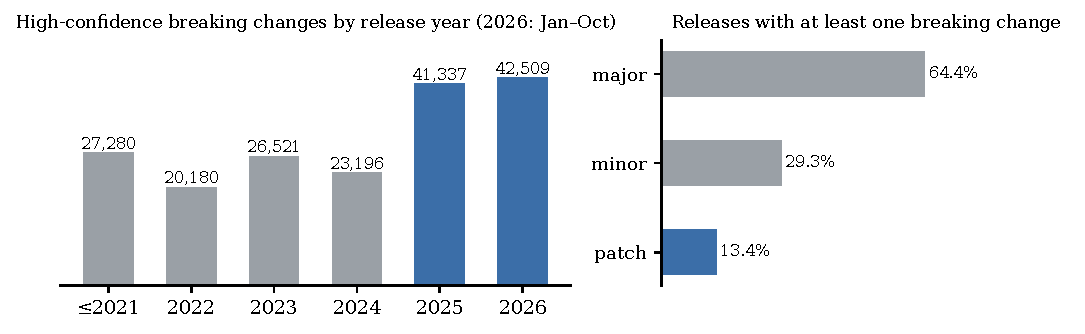
\includegraphics[width=\textwidth]{fig_overview.pdf}
\caption{Left: deduplicated high-confidence breaking changes by year of the breaking release. Because each project's
history is capped at its 80 most recent releases, frequently releasing projects contribute only recent years, so the
rise in 2025--2026 partly reflects coverage. Right: share of release transitions (calendar-versioned releases
excluded) with at least one breaking change, by version increment.}\label{fig:overview}
\end{figure*}

\textbf{Coverage layer.} Absence from the dataset is not proof that a name does not exist. A separate pass over every
analysed wheel records, per module and release range, whether the module was parsed from Python source, only a
\texttt{.pyi} stub ships, the module serves names dynamically (an open module \texttt{\_\_getattr\_\_},
\texttt{globals()} injection, a runtime \texttt{\_\_all\_\_}), or it binds names from compiled extension modules
(289,735 rows in \texttt{module\_coverage}). Each \texttt{api\_history} row carries the resulting
\texttt{coverage\_status}: 79.1\% static, 0.8\% compiled boundary, 17.7\%
dynamic module and 2.3\% stub only. The coverage pass uses a deliberately broad notion of ``dynamic'' (any
\texttt{globals()} use), so it errs toward warning.

\textbf{Integrity.} \texttt{validate\_dataset.py} runs 51 checks on every build: key uniqueness, version order
(including the placeholder rule), interval consistency (no overlaps, indices matching versions, no interval spanning
unanalysed releases), every signature hash resolving, change rows matching their releases, label domains, benchmark
provenance (each pair traces to a breaking change between its two releases), and a recomputation of every headline
count; the released build passes all of them. A regression suite of 158 tests covers each false-positive pattern
found by the audits, and the released files are pinned by SHA-256 in a manifest that the tools verify.

\section{Tools and Benchmark}\label{sec:tools}
\textbf{apidrift-check} parses Python code, resolves imports and simple constructor-based types
(\texttt{df = pd.DataFrame(); df.append(...)}), and checks each referenced path and keyword argument against the
API of the pinned release. By default it reports only names and keywords that were public in \emph{some}
analysed release but not the pinned one, each with a hint (``last present in 1.5.3'', ``accepted up to
1.26.20''). On 1,823 source files of 14 widely used packages, checked against their own installed
dependency versions, it raised 20 findings. Six point to APIs that really are absent in the installed
versions, inside version-guarded or unused code paths. The rest are false alarms: parameters still accepted
through compatibility decorators (e.g.\ SciPy's \texttt{seed}$\to$\texttt{rng} transition), attributes set
dynamically, a method inherited from a compiled base class, and one name that was removed and later re-added outside
the public API. The checker skips \texttt{if TYPE\_CHECKING:} blocks and postponed annotations, which never run; a
strict mode additionally flags names never seen in the API and checks arity. It reads only the Parquet row groups of
the pinned libraries and the signatures they reference: a cold start (one file, one pin) takes 3.1\,s of
CPU and about 326\,MB of memory, and checking all 1,421 files of pandas against its installed
dependencies takes 45.7\,s of CPU on a shared two-core machine. It reads lockfiles (\texttt{uv.lock},
Poetry, \texttt{pylock.toml}, Pipfile), writes SARIF for GitHub code scanning, and ships as an experimental GitHub
Action whose inputs reach the checker only as validated arguments.

\textbf{apidrift-lookup and an MCP server.} \texttt{apidrift-lookup} answers one-line queries offline: the history
of a symbol (\texttt{history pandas DataFrame.append}) and the breaking differences between any two analysed releases
(\texttt{diff flask 2.3.3 3.0.0}), computed from the two API snapshots, each change listed once with its confidence
label. \texttt{apidrift-mcp} exposes these lookups and the checker as read-only tools of a Model Context Protocol
server, so coding agents can consult the record before or after generating code. Every answer carries the coverage
status of the rows it rests on, and a name that is not found is reported with the reminder that absence is weaker
evidence than a recorded change.

\textbf{VersionProbe} contains 10,958 pairs from 583 libraries in the released version. Each pair is one snippet
that is valid in release $A$ and invalid in the next release $B$, derived from a high-confidence
\texttt{removed}, \texttt{param\_removed} or \texttt{param\_renamed} event and verified with the checker in both
directions. Items carry the release date of $B$, so evaluations can be split before and after a model's training
cutoff. A model is asked whether the snippet is valid for the stated version; a constant predictor scores 50\%.
\emph{VersionProbe-verified} is the subset of 492 pairs (984 items, 375 libraries) whose
labels were confirmed at runtime by the benchmark audits of Section~\ref{sec:benchlabels} and that remain in the
released benchmark; it is the split to rank models on.

\section{Validation}\label{sec:validation}
\textbf{Protocol.} Every validation study used \emph{pipeline-isolated, AI-agent-conducted runtime checks}: an agent
(an LLM with shell access, not a human annotator) that never saw the pipeline or the dataset received only the claims
to check, installed the releases in isolated virtual environments, imported modules, walked attributes and compared
\texttt{inspect.signature}, falling back to reading released sources when installation was impossible. The
independence comes from that isolation, not from a separate human researcher, and disputed cases were not
adjudicated by humans; these audits are a systematic, reproducible spot check, not human-annotated ground truth.
Claims were drawn by stratified random sampling (at most two per library). The studies ran on the data version current
at the time; Appendix~\ref{sec:history} lists what changed afterwards.

\subsection{Precision of breaking changes}
Table~\ref{tab:audit} summarizes four audit rounds. Rounds 1 and 2 were \emph{development} audits: they revealed
recurring false-positive patterns (names still reachable after leaving \texttt{\_\_all\_\_}, re-exports of external
objects, lazy module attributes, \texttt{try/except} fallbacks, the \texttt{\_\_x} convention, stub/runtime
disagreement, typing overloads, dynamically generated namespaces, synthetic classes), each fixed generally in the
method of Section~\ref{sec:method}. Rounds 3 and 4 were \emph{held-out} audits on libraries never used in any earlier
audit, study or fix, so they estimate precision out of sample; round 3 ran on v1.0 of the data and round 4 on v1.2.

\begin{table}[t]\centering\small
\caption{Runtime audits of claimed breaking changes.}\label{tab:audit}
\begin{tabular}{@{}lllr@{}}\toprule
Round & Use & Claims (libs) & Result \\\midrule
1 & dev. & 60 & 37\% false pos. \\
2 & dev. & 60 & 25\% false pos. \\
3 & held-out & 100 (53) & high: 88.8\% \\
 & & & medium: 45.0\% \\
4 & held-out & 160 high (134) & 91.9\% \\\bottomrule
\multicolumn{4}{@{}l@{}}{\footnotesize CIs in the text. Round 3 ran on v1.0 data, round 4 on v1.2.}
\end{tabular}\end{table}

In round 3, high-confidence claims were 88.8\% correct (Wilson 95\% CI 80.0--94.0\%, n=80) and
medium-confidence claims 45.0\% (25.8--65.8\%, n=20); removals scored 98.1\%
(n=53) and signature changes 79.2\% (n=24), and all 3 sampled kind
changes were wrong. Round 4 audited 160 new high-confidence claims from 134 further libraries, stratified
into claims that were new in v1.2 (80) and claims unchanged since v1.1 (80). Precision was 91.9\%
overall (CI 86.6--95.2\%): 90.0\% for the new claims and 93.8\% for the unchanged ones; removals scored 91.4\% (n=128) and signature changes 93.8\%
(n=32). Claims checked at runtime were 92.0\% correct (115/125) and claims checked from source 91.4\%
(32/35); in round 3 the source-checked claims, from packages that could not be installed, were much weaker (36.4\%,
4/11, against 97.1\% at runtime). The remaining false positives come from names served by \texttt{\_\_getattr\_\_} or
compiled star imports, circular wildcard imports, stub-only declarations, inheritance from another distribution and
\texttt{**kwargs} that still accept a renamed keyword. The out-of-sample precision estimates for high-confidence
breaking changes are therefore 88.8\% (v1.0) and 91.9\% (v1.2). All samples, verdicts, evidence and the protocol
are published, together with a 200-item kit for repeating the round-4 sample with human labellers.

\subsection{Benchmark labels}\label{sec:benchlabels}
Two samples of VersionProbe pairs were verified by resolving every name and keyword in both releases at runtime
(never executing the snippet). The first (200 pairs, one per library) found 172 correct
(86.0\%, CI 80.5--90.1\%) and led to two exclusions (instance-only attributes, type-checking-only
names). A second, \emph{fresh} sample of 400 pairs was drawn from the benchmark with these exclusions applied (v1.1), restricted to
265 libraries never used in any earlier audit, study or fix: 366 were correct, 91.5\% (CI 88.4--93.9\%);
removals 90.8\% (n=292), removed parameters 96.3\%
(n=54), renamed parameters 90.7\% (n=54). The ``invalid after''
half held in 97.3\% of pairs and the ``valid before'' half in 94.0\%: almost every error is a
name that looks present statically but does not exist at runtime (deleted with \texttt{del}, defined only in an
\texttt{if False:} branch, present only in a stub), plus two pairs built on a placeholder release. The method of Section~\ref{sec:method} handles both causes.

\subsection{Recall and comparison with existing tools}\label{sec:recall}
An agent introspected both releases of 30 random release pairs at runtime and listed 99 breaking changes. Within the
dataset's definition of public API, recall was 87.5\% (14/16, CI 64.0--96.5\%). Over
all runtime-visible changes it was 59.3\% excluding one outlier (\texttt{trio}, whose 72 wrapper methods were
generated at runtime) and 16.2\% including it; most other misses are helper names imported into modules for
internal use. The dataset is thus a high-precision, low-recall record. Table~\ref{tab:tools} scores griffe and AexPy on
the same pairs with the same matching rule. AexPy, which imports every release, finds most runtime-generated changes;
within the shared public-API definition the three methods are close, and what distinguishes the dataset is its scale
and its precomputed history across releases, which needs no installation. The runtime reference set itself is incomplete (some changes found by both this
dataset and AexPy are absent from it), so we report agreement rather than precision for the tools' extra claims.

\begin{table}[t]\centering\small
\caption{Breaking changes detected on the 30 recall pairs (runtime reference set).}\label{tab:tools}
\begin{tabular}{@{}lccc@{}}\toprule
 & PyPI API Drift & griffe & AexPy \\\midrule
Within API-Drift definition & 14/16 & 12/16 & 13/16 \\
Runtime-visible, w/o trio & 16/27 & 12/27 & 20/27 \\
All runtime-visible & 16/99 & 12/99 & 90/99 \\
Pairs analysed & 30 & 30 & 29 \\
Median s / pair & 2.1 & 1.3 & 62.7 \\\bottomrule
\multicolumn{4}{@{}l@{}}{\footnotesize Time per pair: extracting both releases (range reads; griffe downloads}\\
\multicolumn{4}{@{}l@{}}{\footnotesize wheels; AexPy installs both releases). One AexPy pair ran out of memory.}\\
\multicolumn{4}{@{}l@{}}{\footnotesize trio: one library whose 72 wrapper methods are generated at runtime.}
\end{tabular}\end{table}

\subsection{Real upgrade failures}
\textbf{Pilot.} An agent ran the test suites of 12 real projects (9 breaking dependency upgrades, 3 controls) before and
after the upgrade and found 12 API-caused failures. \texttt{apidrift-check} produced 7 findings, all
real, with none on the old environments or controls, but predicted only 4 of the failures.

\textbf{Unseen upgrades.} We then froze the checker and the v1.0 data and had two agents, who never ran the checker, collect
35 new cases (25 expected breaks, 10 controls, 27 libraries, including compiled
packages and lazily loaded APIs). 32 were scored (the other library versions were never analysed, and the
checker reports that instead of guessing). With the frozen checker, 63 of 68 findings pointed at
real incompatible code (92.6\%, CI 83.9--96.8\%), including code that the tests never exercise, and it
predicted 9 of 18 API-caused test failures (50.0\%, CI 29.0--71.0\%); it raised findings on
3 of 14 upgrades with no API failure (two of them real but untested incompatibilities).
With the released data and checker it predicts 14 of 18, and 93 of its
106 findings match what the agents observed. These figures are in-sample, because several rules of
Section~\ref{sec:method} were introduced after studying these misses; the frozen figures are the out-of-sample ones.
The remaining misses include a module re-exporting an external package (\texttt{lxml.html.clean}), dunder names
(skipped by design), a call through a subclass, and NumPy's \texttt{float} in 1.24.0, which disappeared without an
explicit rejection and so cannot be proven absent statically.

\section{Does the Record Help Code Models?}\label{sec:models}
\subsection{Classification baseline}
On VersionProbe-verified, items were shuffled and asked one at a time (``is this snippet valid in exactly version
$v$?''). A Claude model (\texttt{claude-opus-5-5}), run as an agent allowed only to read the questions and write
answers, scored 58.4\% item accuracy (CI 55.3--61.5\%) and 26.6\% pair accuracy from its own
knowledge, against 50\% and 0\% for a constant answer. It accepted most valid snippets (72.8\%) but recognized
only 44.1\% of invalid ones, and was weaker on changes released after its training cutoff (52.1\%,
n=96, against 59.1\%). Given API history retrieved from the dataset for every name and keyword
in the snippet (the releases in which each existed or was accepted; no label), it scored 100.0\%. This is
essentially an oracle condition: it shows only that the answer is in the record when retrieved, not that models
benefit in general, which the repair experiment tests.

\subsection{Code repair}
We ran a preregistered repair experiment (task list hashed before any model output). 143 real breaking changes
from 109 libraries (removals with a recorded new location, renamed and removed parameters; 7 more tasks were
excluded because the original snippet already resolved and bound in the new release) were given to the model as code
written for the old release, with the instruction to update it for the new release while keeping its purpose. Three
conditions: closed book; \emph{documentation}, an API reference page for the imported module(s) generated with griffe
from the new release's wheel; and \emph{PyPI API Drift}, the dataset's history, recorded change and new signatures for
the snippet's names. Each answer was checked at runtime in an environment with only the new release installed (every
name resolves and every call's arguments bind to its signature; the call is not executed, and missing required
arguments are not checked), and a separate model, blind to the condition, judged whether it preserved the snippet's
intent rather than deleting or substituting the call. ``Success'' means both checks passed under this protocol; it is
not evidence of behavioural equivalence, and the intent check is an AI judgement, not a human verification.

\begin{table}[t]\centering\small
\caption{Code repair on 143 real breaking changes (preregistered run, \texttt{claude-opus-5-5}).}\label{tab:repair}
\begin{tabular}{@{}lccc@{}}\toprule
 & Closed book & Docs & API Drift \\\midrule
API-compatible & 58.7\% & 69.9\% & 80.4\% \\
Intent (AI judge) & 93.0\% & 86.0\% & 88.1\% \\
\textbf{Both} & \textbf{56.6\%} & \textbf{60.1\%} & \textbf{68.5\%} \\
\quad removed parameter & 52.3\% & 56.8\% & 70.5\% \\
\quad renamed parameter & 57.1\% & 73.8\% & 76.2\% \\
\quad moved/removed name & 59.7\% & 52.6\% & 61.4\% \\\bottomrule
\end{tabular}\end{table}

With API history the model succeeded on 68.5\% of tasks (CI 60.5--75.6\%), against 56.6\% closed book
(exact McNemar $p=0.0115$; 29 tasks fixed only with the history, 12 only without) and
60.1\% with documentation ($p=0.0428$; 21 vs 9). The gain comes from validity: answers
written against the dataset's record were API-compatible far more often, while slightly more were judged unfaithful,
mostly where a ``still available as'' hint pointed to a same-named but different object. Both preregistered
hypotheses hold and survive a Holm correction for the two comparisons (adjusted $p=0.023$ and
$0.0428$); under the more conservative Bonferroni correction the documentation comparison would not
($p=0.0856$). In a post-hoc sensitivity check (not preregistered), every answer was re-verified in fresh
environments with full argument binding (\texttt{Signature.bind} instead of \texttt{bind\_partial}, so a missing
required argument fails); the re-run reproduced every
preregistered verdict, and full binding removed 2 successes (1 closed book, 1
documentation, 0 API Drift), giving 55.9\%, 59.4\% and 68.5\% ($p=0.0064$ and
$p=0.0294$).

\subsection{Replication across models}
We then repeated both experiments, unchanged, with three more Claude models (\texttt{claude-sonnet-5-5},
\texttt{claude-haiku-5-5} and \texttt{claude-fable-5-1}): the same 984 VersionProbe-verified items, and the same 150
repair tasks (143 scored after the same exclusion), runtime check and blind judge (\texttt{claude-opus-5-5}),
with every answer verified under both the partial and the full binding check. The ordering closed book $<$ documentation $<$ API Drift holds for every model
(Table~\ref{tab:models}). With API history the models end up close together: closed-book success ranged from 7.0\% to
56.6\% (the smallest model left 88.7\% of snippets unchanged without help), but with the history
all four reached 68.5\%--69.9\%. API history beat documentation for all
4 models, with unadjusted exact McNemar $p<0.05$ for 3 (the exception has
$p=0.071$), and closed book for
all 4; full binding removed 0 API Drift successes. On VersionProbe the smaller models
are close to the 50\% of a constant answer. The models are of one family, so this replicates the protocol, not the
result across model families; with 143 tasks per model, each rate has a 95\% interval of roughly $\pm$7--8 points.

\begin{table}[t]\centering\small
\caption{Replication: VersionProbe-verified (closed book) and code repair success per condition.}\label{tab:models}
\setlength{\tabcolsep}{2.5pt}
\begin{tabular}{@{}lcccccc@{}}\toprule
 & \multicolumn{2}{c}{VersionProbe} & \multicolumn{3}{c}{Repair success} & $p$ vs \\
Model & item & pair & closed & docs & API Drift & docs \\\midrule
opus-5-5$^\ast$ & 58.4\% & 26.6\% & 56.6\% & 60.1\% & \textbf{68.5\%} & 0.043 \\
sonnet-5-5 & 54.3\% & 18.3\% & 42.0\% & 56.6\% & \textbf{69.2\%} & 0.0029 \\
haiku-5-5 & 49.6\% & 9.2\% & 7.0\% & 46.2\% & \textbf{68.5\%} & $<$0.0001 \\
fable-5-1 & 56.5\% & 22.4\% & 49.7\% & 62.2\% & \textbf{69.9\%} & 0.071 \\\bottomrule
\multicolumn{7}{@{}l@{}}{\footnotesize $^\ast$preregistered run; $p$: exact McNemar, API Drift vs documentation.}\\
\end{tabular}\end{table}

\section{Findings}\label{sec:findings}

\textbf{Semantic versioning.} Excluding calendar-versioned releases, 64.4\% of major, 29.3\% of minor and 13.4\% of patch increments include at least one
breaking change. 840 of the 1,869 libraries with analysed releases shipped at least one
breaking patch release. These rates count any public-API break, including rarely used members, so they overstate how often a typical user
is affected (consistent with the Maven observation that most breaking changes affect code few clients
use~\cite{ochoa2022}), while missing the breaks that static analysis cannot see (Section~\ref{sec:recall}). A version bump is not a promise, so we also split projects by the policy their PyPI
description states (pattern match, every match reviewed by hand): 54 say they follow SemVer,
2 say they do not, 61 use calendar versions, and 1,755 state nothing there. Among the
SemVer projects' stable ($\geq$1.0) releases, 16.7\% of 707 patch releases
(17 of 40 projects) and 24.5\% of minor releases contain a high-confidence
breaking change; these are candidate SemVer violations, subject to the audited precision and to the caveat above.

\textbf{Deprecation before removal.} Only 4.8\% of removed functions, classes and methods carried a
statically detectable deprecation marker (decorator, docstring directive or unconditional warning) in an earlier
analysed release. Deprecation is often communicated through changelogs or conditional warnings rather than
markers that tools can see.

\textbf{Recency.} 83,846 high-confidence breaking changes were released from 2025 onward
(Fig.~\ref{fig:overview}; the per-year counts are affected by the 80-release cap). Code models whose training data
predates them cannot know these changes without retrieval, which motivates checking generated code against
version-specific API records.

\section{Limitations}
PyPI API Drift is a high-precision, low-recall record, not complete ground truth. The analysis is static: compiled
extensions are visible only through stubs, parameters altered by decorators are not modelled, and names created at
runtime are often missing. This matters most for the libraries users try first: among the 100 most-downloaded
libraries, 74.8\% of API-history rows come from fully static modules (19.8\% dynamic,
5.3\% compiled boundary), against 86.3\% for ranks 101--500; the
\texttt{coverage\_status} column marks every such row. Inheritance from classes in other distributions is not
resolved (these cases are labelled medium). The history covers at most the 80 most recent final releases per
project, so year-over-year counts are shaped by the cap, and release order follows version numbers. Behavioural
changes with unchanged signatures are out of scope, and statically detectable deprecation markers cover only a small
share of removals. All validation used samples checked by AI agents isolated from the pipeline, without human
adjudication; the released labelling kit allows this to be repeated by people. The held-out audits ran on v1.0 and v1.2; the v1.3
changes (Appendix~\ref{sec:history}) both added and relabelled claims and have not been re-audited. Recall depends on
the public-API definition, and a tool that imports releases (AexPy) finds far more of the runtime-visible changes.
The model experiments use 4 models of one family; the repair study checks names and signatures at
runtime and intent with an AI judge, not program behaviour. The checker infers types only for objects constructed and
assigned in the same scope, follows \texttt{super()} calls into library base classes but no other calls through
subclasses, and never flags private or dunder names, which limits its recall on real upgrades.

\section{Availability}
Code and tools (Apache-2.0), validation material and the benchmark:
\url{https://github.com/pushkardg/pypi-api-drift}. Data (CC BY 4.0, release 2026.10-v1.3, with SHA-256 manifest):
\url{https://huggingface.co/datasets/pushkar87dg/pypi-api-drift}. The pipeline is incremental and is intended to be
re-run regularly, so new releases are added as they appear.

\section*{Acknowledgment}
AI assistance was used for parts of the data-processing code and for editing this manuscript; the author reviewed
all content and is responsible for it.

\balance
\begin{thebibliography}{9}\footnotesize
\bibitem{versicode} T.~Wu \emph{et al.}, ``VersiCode: Towards version-controllable code generation,'' arXiv:2406.07411, 2024.
\bibitem{gitchameleon} N.~Islah, J.~Gehring, D.~Misra, E.~Muller, I.~Rish, T.~Y.~Zhuo, and M.~Caccia, ``GitChameleon: Unmasking the version-switching capabilities of code generation models,'' arXiv:2411.05830, 2024.
\bibitem{gitchameleon2} D.~Misra \emph{et al.}, ``GitChameleon 2.0: Evaluating AI code generation against Python library version incompatibilities,'' arXiv:2507.12367, 2025.
\bibitem{wang2024deprecated} C.~Wang, K.~Huang, J.~Zhang, Y.~Feng, L.~Zhang, Y.~Liu, and X.~Peng, ``LLMs meet library evolution: Evaluating deprecated API usage in LLM-based code completion,'' arXiv:2406.09834, 2024.
\bibitem{griffe} T.~Mazzucotelli, ``griffe: Signatures for entire Python programs,'' \url{https://mkdocstrings.github.io/griffe/}, 2026.
\bibitem{aexpy} X.~Du and J.~Ma, ``AexPy: Detecting API breaking changes in Python packages,'' in \emph{Proc. IEEE 33rd Int. Symp. Software Reliability Engineering (ISSRE)}, 2022, pp.~470--481.
\bibitem{raemaekers2014} S.~Raemaekers, A.~van~Deursen, and J.~Visser, ``Semantic versioning versus breaking changes: A study of the Maven repository,'' in \emph{Proc. IEEE 14th Int. Working Conf. Source Code Analysis and Manipulation (SCAM)}, 2014, pp.~215--224.
\bibitem{ochoa2022} L.~Ochoa, T.~Degueule, J.-R.~Falleri, and J.~Vinju, ``Breaking bad? Semantic versioning and impact of breaking changes in Maven Central,'' \emph{Empirical Software Engineering}, vol.~27, 2022.
\end{thebibliography}

\appendix
\section{Release History}\label{sec:history}
The data was revised as audits and reviews exposed defects; each version was rebuilt in full and passed the integrity
checks.

\textbf{Which version each study used.} v1.0: precision audits 1--3 (rounds 1--2 on development builds), the
first benchmark-label sample, the upgrade pilot, the frozen unseen-upgrade study and the checker false-alarm test. v1.1:
the fresh 400-pair benchmark audit and the classification baseline on VersionProbe-verified. v1.2: precision audit 4,
the code-repair experiment and its replications (history supplied from v1.2), the tool comparison and the re-scored
recall study (unchanged from its first run). v1.3: the released counts, figures and benchmark, and the re-scored
unseen-upgrade results.

\textbf{v1.0 to v1.1.} 77 renames of positional-only parameters had been labelled breaking; 369
constructor-signature events concerned decorator-built classes (now medium, signature dropped from 9,373
history rows); intervals of two projects extended over releases too large to analyse (342,126 rows); module-to-distribution mapping used only the latest release; the coverage layer was added.

\textbf{v1.2.} Three over-cautious rules hid removals: any use of \texttt{globals()} marked a module as dynamic (NumPy
2.0's \texttt{bool8}), a runtime-built \texttt{\_\_all\_\_} blocked attribute checks (SciPy's \texttt{simps}), and
star-import chains were abandoned (NetworkX); names deleted with \texttt{del} were kept. After re-extraction,
high-confidence breaking changes went from 175,221 to 181,950, 82 VersionProbe
pairs whose change no longer held were dropped (including 4 that the fresh benchmark audit had
judged wrong), and the round-3 claims still labelled high confidence under the new rules (73 of 80) were
94.5\% correct (in-sample). The checker gained \texttt{super()} checks.

\textbf{v1.3.} 5 placeholder releases were removed (1,761 change events, 6
VersionProbe pairs); module \texttt{\_\_getattr\_\_} containers are followed (56 libraries re-extracted,
27,360 more public paths); and 1,123 high-confidence removals dated by provability became medium,
with 66 VersionProbe pairs dropped. High-confidence breaking changes went from 181,950 (v1.2) to
181,023; the unseen-upgrade results were unchanged.

\end{document}
